\documentclass{standalone}
\usepackage{tikz, pgfplots}

\begin{document}
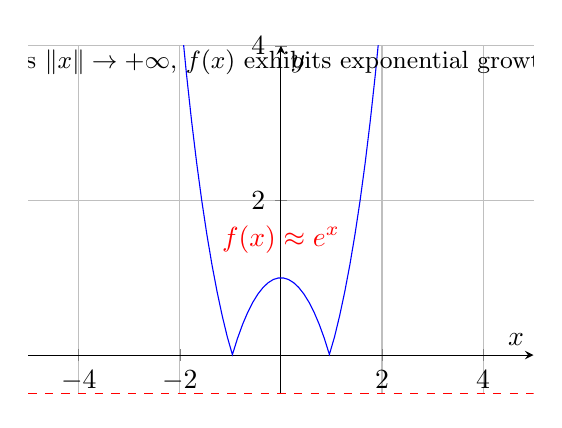
\begin{tikzpicture}
    \begin{axis}[
        axis lines=middle,
        xlabel=$x$,
        ylabel=$y$,
        ymin=-0.5,
        ymax=4,
        xmin=-5,
        xmax=5,
        domain=-5:5,
        samples=100,
        grid=major,
        width=8cm,
        height=6cm
    ]
        % Plot the function f(x) = |e^x + e^{-x} - 3|
        \addplot[blue] {abs(exp(x) + exp(-x) - 3)};
        
        % Highlight the regions where the function exhibits exponential growth
        \draw[dashed, red] (axis cs:-5,-0.5) -- (axis cs:5,-0.5);
        \node at (axis cs:0,1.5) [red] {$f(x) \approx e^x$};
        
        % Add labels and title
        \node at (axis cs:0,-0.7) [below] {\small $f(x) = |e^x + e^{-x} - 3|$};
        \node at (axis cs:0,3.5) [above] {\small As $\|x\| \to +\infty$, $f(x)$ exhibits exponential growth};
    \end{axis}
\end{tikzpicture}
\end{document}